For the last architecture, coalitions, the same tasks are handled again. To start a coalition architecture, start 
\textit{3\_CoaltionController.sh}.
Now, splitting n \acp{uav} into n coalitions. Each coalition will take on a subarea, with its tasks, to complete.

In this example 7 \acp{uav} are split up into 4 coaltions, with the last only containing 1 \acp{uav}.

\begin{figure}[ht]
    \centering
    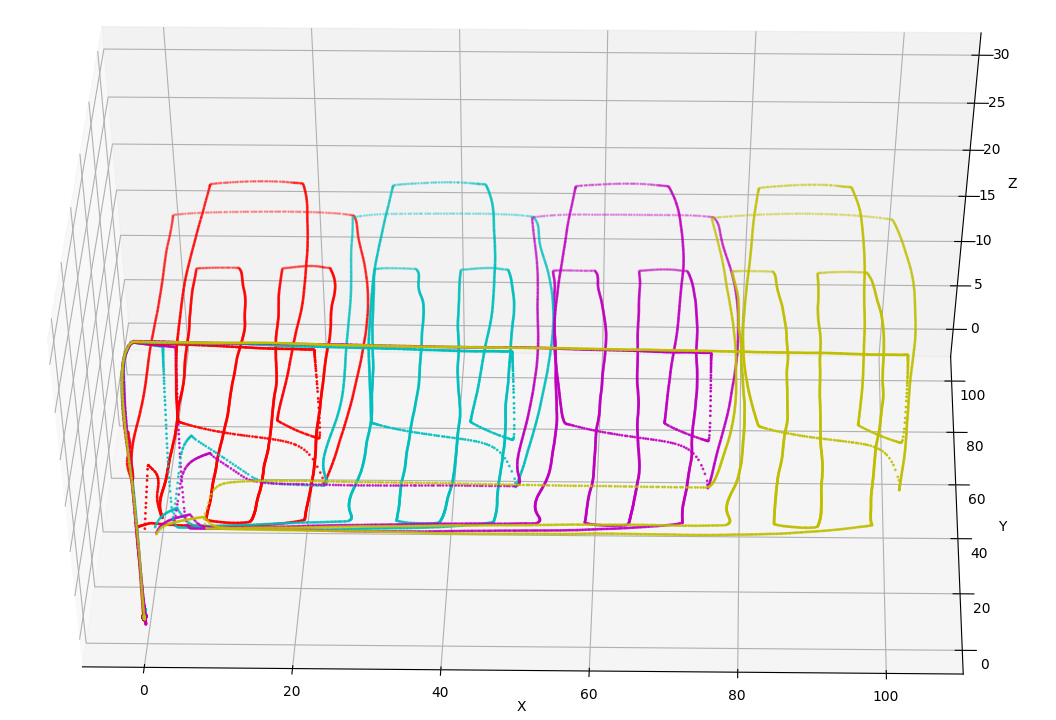
\includegraphics[scale=0.4]{coalition_size_2/coalitionFullSideView.png}
    \caption[coalition flight patters]{coalition flight patters}
\end{figure}

Each coaltion completed a subarea with all its tasks. 

\newpage
\begin{figure}[ht]
    \centering
    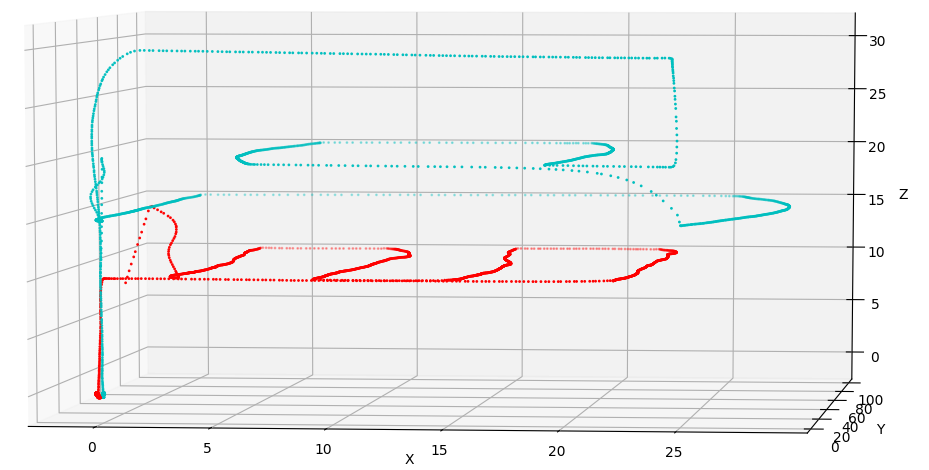
\includegraphics[scale=0.4]{coalition_size_2/coalition1_unique.png}
    \caption[coalition flight patters]{coalition flight patters}
\end{figure}

Examining the first coalition, it can be seen that one \acs{uav} did two tasks en the second \acs{uav} did only one.

\begin{figure}[ht]
    \centering
    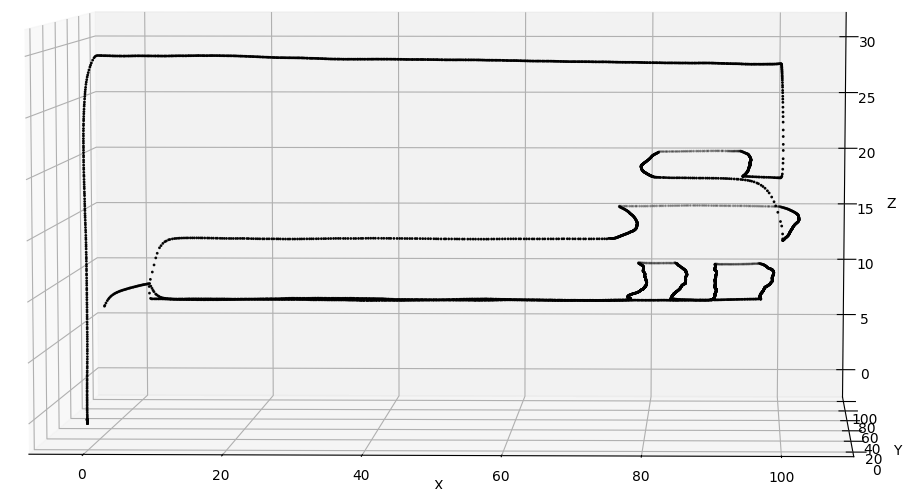
\includegraphics[scale=0.4]{coalition_size_2/coalition4_unique.png}
    \caption[coalition flight patters]{coalition flight patters}
\end{figure}

The last team, again only containing one \acs{uav}, completed its subarea on its own and did all the tasks.
